\documentclass[11pt, addpoints, answers]{exam}
%\documentclass[12pt, addpoints]{exam}
\usepackage{tikz}
\usetikzlibrary{graphs,positioning}
\usepackage{amsmath, amssymb}
\usepackage{xcolor}
\usepackage{tikz}
\usepackage{enumerate}
\usepackage{graphicx}
\usepackage{tabularx}
\usepackage{algorithm}
\usepackage{algpseudocode}

\usepackage{graphics}
\usepackage{tikz}
\usepackage{tikz-qtree}
\usepackage{drawstack}

\usetikzlibrary{graphs}
\tikzset{every tree node/.style={minimum width=2em,draw,circle},
	blank/.style={draw=none},
	edge from parent/.style=
	{draw,edge from parent path={(\tikzparentnode) -- (\tikzchildnode)}},
	level distance=1.2cm}

\newcommand{\red}[1]{\textcolor{red}{#1}}
\newcommand{\blue}[1]{\textcolor{blue}{#1}}

% For inserting code snippets.
\usepackage{listings}
\lstset{
	columns = fixed,
	basewidth = {0.5em},
	breaklines = true,
	backgroundcolor = \color{white},
	keywordstyle = \color[RGB]{40, 40, 255},
	numberstyle = \footnotesize\color{darkgray},
	commentstyle = \ttfamily\color{violet},
	basicstyle = \ttfamily,
	stringstyle = \ttfamily\color[RGB]{128, 0, 0},
	showstringspaces = false,
	language = {[11]C++},
	escapechar = \@
}
\lstnewenvironment{cpp}[1][]{\lstset{language = {[11]C++}, #1}}{}

\renewcommand{\baselinestretch}{1.15}
\setlength{\parskip}{1.25\baselineskip}

\newcolumntype{C}[1]{>{\centering\arraybackslash}p{#1}}
\definecolor{lightgray}{gray}{0.9}

% headers, footers, titles
\title{CS101A(H) Homework 8}
\author{}
\date{Due date: December 30, 2025, at 20:00 p.m.}

% formats of questions, choices, points, etc.
\qformat{\bf\thequestion. (\totalpoints\ points) \thequestiontitle\hfill}
\pointname{'}
\CorrectChoiceEmphasis{\bf\color{blue}}
\SolutionEmphasis{\color{blue}}

% We frequently use this font.
\newcommand{\ttt}{\texttt}
\newcommand{\bluett}[1]{\textcolor{blue}{\ttt{#1}}}

\begin{document}
	
	\maketitle
	
	The total score of this assignment is 30 points.
	
	\textbf{Notes: } \textbf{Unless otherwise stated, always express your final asymptotic bounds using} \(\boldsymbol{\Theta(\cdot)}\) \textbf{notation for tight complexity, not just} \(O(\cdot)\) \textbf{or} \(\Omega(\cdot)\).  
	All answers must be written \textbf{inside the provided answer boxes} and \textbf{in English}. When submitting, match your solutions to the problems correctly in Gradescope. No late submission will be accepted. Failure to follow these rule may result in partial or full loss of credit.
	
	
	
	\paragraph{Usage of AI.}
	The use of AI tools for searching information or obtaining assistance on this homework is strictly prohibited. All solutions must be derived from your own understanding and effort. Submissions will be reviewed carefully, and any indication of reliance on AI-generated content will result in severe penalties.
	
	\paragraph{Academic Integrity.}
	This course upholds the highest standards of academic integrity. Any form of academic dishonesty, including plagiarism, unauthorized collaboration, or the use of prohibited resources such as AI tools, will be treated as a serious violation. Such actions not only undermine your own learning but also violate university policies. 
	
	\begin{questions}
		
		\newpage
		\begin{table}[h]
			\centering
			\caption{Fill answers here}
			\begin{tabular}{|C{1.8cm}|C{1.2cm}|C{1.2cm}|C{1.2cm}|C{1.2cm}|C{1.2cm}|C{1.2cm}|C{1.2cm}|C{1.2cm}|C{1.2cm}|}
				\hline
				question  & 1 & 2 & 3 & 4  \\
				\hline
				answer & & & &   \\
				\hline
				%question & 10 & 11 & 12 & 13 & 14  \\
				%\hline
				%answer & & & & &  \\
				%\hline
			\end{tabular}
		\end{table}
		
%==================== Single Choice Questions ====================

\titledquestion{Single Choices}

Each question has {\textbf{exactly one}} correct answer. Select the best answer.

\begin{parts}
	
	%---------- Q1 ----------
	\part[2] We run the Floyd-Warshall algorithm on a simple graph without negative cycles with $3n$ vertices $v_1, \ldots, v_{n}, \ldots, v_{2n}, \ldots,  v_{3n}$. Suppose all three loops $(k, i, j)$ are iterated from $1$ to $3n$. After running at least how many iterations of the out-most loop $k$, it is ensured to find the shortest path between $v_{2n}$ and $v_{3n}$?
	\begin{choices}
		\choice $2n-1$
		\choice $2n$
		\choice $3n-1$
		\choice $3n$
	\end{choices}
	
	% ---------------Q2--------------
	\part[2] Which of the following statements is \textbf{TRUE}?
	\begin{choices}
		\choice Bellman-Ford algorithm can find the shortest path for negative-weighted directed graphs, while the Dijkstra algorithm may fail.
		\choice The run time of the Bellman-Ford algorithm is $O(|V||E|)$, which is more time-consuming than the Dijkstra algorithm with heap implementation.
		\choice The A* graph search algorithm with an admissible heuristic will always return an optimal solution if it exists.
		\choice Floyd-Warshall algorithm can always give the correct shortest distance between any two vertices in directed graphs with negative weights.
	\end{choices}
\end{parts}

		
%==================== Multiple Choice Questions ====================

\titledquestion{Multiple Choices}

Each question has {\textbf{one or more}} correct answers.  
Select \textbf{all} correct answers. You will receive \textbf{no credit} if you select any wrong choice for a question.

\begin{parts}
	
	%---------- Q3----------
	\part[3] Which of the following statements is/are \textbf{TRUE}?
	\begin{choices}
		\choice Dijkstra algorithm can find the shortest path in any DAG.
		\choice If we use the Dijkstra algorithm, whether the graph is directed or undirected does not matter.
		\choice At each iteration of the Dijkstra algorithm, we pop the vertex with the shortest current distance to the start vertex, while in the Prim algorithm, we pop the vertex with the shortest distance to the current minimum spanning tree.
		\choice In directed graph $G = (V, E)$, if $(s, v_1, v_2, v_3, v_4, t)$, where $s, v_i, t \in V$ , is the shortest path from $s$ to $t$ in $G$, then $(v_1, v_2, v_3, v_4)$ must be the shortest path from $v_1$ to $v_4$ in $G$.
	\end{choices}
	
	% ---------- Q4 -------------
	\part[3] Which of the following is/are \textbf{TRUE}?
	\begin{choices}
		\choice Dijkstra algorithm can be viewed as a special case of the A* Graph Search algorithm where the heuristic function from any vertex $u$ to the terminal $z$ is $h(u, z)=0$.
		\choice For two graphs $G_1=(V_1,E_1),G_2=(V_2,E_2)$ such that $|V_1|=|V_2|$ but $|E_1|>|E_2|$, the Floyd-Warshall algorithm costs more time on $G_1$ than $G_2$.
		\choice In A* graph search algorithm with a consistent heuristic function, if vertex $u$ is marked visited before $v$, then $d(u)+h(u)\leq d(v)+h(v)$, where $d(u)$ is the distance from the start vertex to $u$.
		\choice In a DAG with probably negative edge weights, Bellman-Ford algorithm is guaranteed to find the shortest path from source $s$ to any vertex if it can be reached from $s$.
	\end{choices}
	
\end{parts}

		\newpage
\titledquestion{A star}

Logan is doing an A* \textbf{graph search} from $S$ to $T$ on the graph below. Edges are labeled with weights.

The exploration order follows in their lexicographical order. (For example, $S \to X \to A$ would be expanded before $S \to X \to B$, and $S \to A \to Z$ would be expanded before $S \to B \to A$.
\begin{table}[!ht]
	\begin{minipage}[b]{0.6\linewidth}
		\centering
		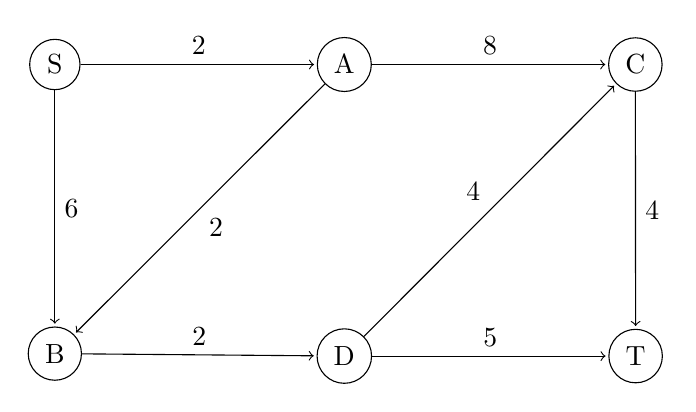
\begin{tikzpicture}[shorten >=1pt,node distance=2cm,auto]
			\node[circle,draw] (S) {S};
			\node[circle,draw] (A) [right=3cm of S] {A};
			\node[circle,draw] (B) [below=3cm of S] {B};
			\node[circle,draw] (C) [right=3cm of A] {C};
			\node[circle,draw] (D) [below=3cm of A] {D};
			\node[circle,draw] (T) [right=3cm of D] {T};
			\path[->]
			(S) edge node {2} (A)
			(A) edge node {2} (B)
			(S) edge node {6} (B)
			(B) edge node {2} (D)
			(D) edge node {5} (T)
			(A) edge node {8} (C)
			(D) edge node {4} (C)
			(C) edge node {4} (T);
		\end{tikzpicture}
	\end{minipage}
	\begin{minipage}[b]{0.35\linewidth}
		\centering
		\begin{tabular}{|r|l|l|l|l|l|l|}
			\hline
			Node & S & A & B & C & D& T \\ \hline
			Heuristic & $11$ & $9$ & $12$ & $4$ & $5$ & $0$ \\ \hline
		\end{tabular}
		\caption{The initial heuristic value}
		\label{tab:heuristic}
		\begin{table}[H]
			\centering
			\begin{tabular}{|r|l|l|l|l|l|l|}
				\hline
				Node & S & A & B & C & D& T \\ \hline
				Heuristic & $10$ & $6$ & $4$ & $2$ & $3$ & $0$ \\ \hline
			\end{tabular}
			\caption{The new heuristic value}
			\label{tab:new}
		\end{table}
	\end{minipage}
\end{table}\\

\begin{parts}
	\part[3] He first uses the heuristic value in the Table \ref{tab:heuristic} but finds it does not work well. That's because the given heuristic values are:
	\begin{choices}
		\choice Admissible but not consistent
		\choice Consistent but not admissible
		\choice Neither admissible nor consistent
	\end{choices}
	\part Logan decides to modify the heuristic.
	\begin{subparts}
		\subpart[3] He first gives out a new heuristic as in Table \ref{tab:new} above, please check whether the heuristic meets both admissibility and consistency (Write `Yes' or `No' for this). \\
		\textbf{If so}, write down the path from $S$ to $T$ returned by $A^*$ graph search (in the form of nodes, e.g. $S\to A \to C \to T$ should be written as $SACT$). \\
		\textbf{Otherwise}, give out a contradiction that will lead admissibility or consistency to fail (in the form of `Admissibility/Consistency' and its corresponding inequality. \\
		e.g. If consistency fails on $A\to C$, write `Consistency, $h(C) + 8 < h(A)$', here $8$ corresponds to $w(A, C)$.).
		\begin{solution}

		\end{solution}
		
		\newpage
		\subpart[4] He finds that he can modify the heuristic of \textbf{only one node} to meet admissibility and consistency from the initial heuristic values in Table \ref{tab:heuristic}. Find the node and corresponding heuristic value for the chosen node. Justify your answer by stating the equalities obtained from admissibility and consistency.
		\begin{solution}
			
		\end{solution}
	\end{subparts}
	
\end{parts}
		
		\newpage
\titledquestion{Negative Cycle Detection}
The \textbf{inf($\infty$)} mentioned in this problem could be regarded as a pre-defined large enough constant. The graph mentioned in this problem is a simple directed graph. Please write down your codes in \textbf{standard C++}.

\begin{parts}
	\part Consider the following implementation of the Floyd-Warshall algorithm. Suppose $W$ is the adjacency matrix of the graph, and assume that $W_{ij}=\infty$ where there is no edge between vertex $i$ and vertex $j$, and assume $W_{ii}=0$ for every vertex $i$. And other $W_{ij}$ are the weights of the edge between vertex $i$ and vertex $j$.  The array `graph' passed into the function is the adjacency matrix $W$.
	
	\begin{cpp}
bool DetectNegCycle_Floyd(const int graph[][V])
{
	int dist[V][V];
	
	for (int i = 0; i < V; ++i)
	for (int j = 0; j < V; ++j)
	dist[i][j] = graph[i][j];
	
	for (int k = 0; k < V; ++k)
	for (int i = 0; i < V; ++i)
	for (int j = 0; j < V; ++j)
	if (dist[i][j] > dist[i][k] + dist[k][j])
	dist[i][j] = dist[i][k] + dist[k][j];
	
	_____________________________________
	_____________________________________
	_____________________________________
	_____________________________________
	
	return false;
}
	\end{cpp}
	
	\begin{subparts}
		
		\subpart [2] Consider the three loop lines in the Floyd-Warshall algorithm: lines $9, 10$, and $11$. Which pair(s) of these lines can be swapped without affecting the correctness of the algorithm? List all possible pairs of lines that can be swapped.
		
		\begin{solution}

		\end{solution}
		
		\subpart[4] Add some codes in the blank lines to detect whether there are negative cycles in the graph. (You may not use all blank lines, or you can add more lines.)
		
		\begin{solution}
			\begin{cpp}
_____________________________________
_____________________________________
_____________________________________
_____________________________________
			\end{cpp}
		\end{solution}
	\end{subparts}
	
	\part[4] Consider the following implementation of the Bellman-Ford algorithm. The `edge' structure is used to represent the edges of the graph, with its elements $u$, $v$, and $w$ denoting an edge from node $u$ to node $v$ and its corresponding weight $w$.
	
\begin{cpp}
struct edge
{
	int u, v, w;
};

bool detectNegCycle_BellmanFord(const std::vector<edge>& Edge, int s)
{
	int dist[V];
	
	for (int i = 0; i < V; ++i)
	dist[i] = inf;
	dist[s] = 0;
	
	for(i = 1; i <= V - 1; ++i)
	{
		for(const auto& e : Edge)
		if (dist[e.v] > dist[e.u] + e.w)
		dist[e.v] = dist[e.u] + e.w;
	}
	
	_____________________________________
	_____________________________________
	_____________________________________
	_____________________________________
	
	return false;
}
\end{cpp}
	
	Add some codes in the blank lines to detect whether there are negative cycles in the graph. (You may not use all blank lines, or you can add more lines.)
	
	\begin{solution}
		\begin{cpp}
_____________________________________
_____________________________________
_____________________________________
_____________________________________
		\end{cpp}
	\end{solution}
	
\end{parts}
		
	\end{questions}
	
\end{document}